%!TEX encoding = UTF-8 Unicode
%!TEX TS-program = pdflatex

%%% --- PREAMBLE --- %%%

\documentclass[a4paper,11pt]{article}

\usepackage[italian]{babel}
\usepackage[left=2cm,right=2cm,top=2cm,bottom=2cm]{geometry}
\usepackage[T1]{fontenc} % OT1: basic, T1: western, T3 and T5: exotic, T4: lots of characters but WORSE READABILITY
\usepackage[utf8x]{inputenc} % utf8x supports more characters than utf8
\usepackage{graphicx} % import PNG, JPG and PDF with \includegraphics
\usepackage[usenames,table]{xcolor} % \color
\usepackage{amssymb}
\usepackage{amsmath}
\usepackage{amsfonts}
\usepackage{mathtools} % (!! PLACE BEFORE hyperref !!)
\usepackage{xfrac} % \sfrac
\usepackage{cancel} % \cancel \cancelto
\usepackage{hyperref} % interactive links in TOC, URLs and references
% Bob \usepackage[version=3]{mhchem} % \ce (chemical formula)
\usepackage{siunitx} % \num \si \SI
\usepackage{alltt} % {alltt} (like verbatim but with commands)
\usepackage{moreverb} % {listing}
\usepackage{listings} % {lstlisting}
\usepackage[overload]{textcase} % fixes \MakeUppercase and \MakeLowercase
\usepackage[normalem]{ulem} % \uline \uwave \sout \xout
\usepackage{enumerate} % adds options for {enumerate}
\usepackage{paralist} % inline lists with {inparaenum}
\usepackage[official]{eurosym} % \euro
\usepackage{tabu} % {tabu} (like {tabular} with improvements)
\usepackage{layout} % layout description
\usepackage{multicol} % {multicols}
\usepackage{lipsum} % filling text generator with \lipsum
\usepackage[section]{placeins} % inhibits float figures from trepassing a section boundary
\usepackage{subfig} % \subfloat to be used inside {figure}
\usepackage{wrapfig} % {wrapfigure} (like {figure} but allows text to flow on its sides)
\usepackage{ifthen} % \ifthenelse
\usepackage{calc}
\usepackage{array}
\usepackage{multirow}
\usepackage{booktabs} % \toprule, \midrule, \bottomrule

\graphicspath{ {../Figs-Tabs/} } % graphics search directories
\setcounter{tocdepth}{1} % -1: part, 0: chapter, 1: section, 2: subsection, 3: subsubsection

\lstset{ %
	language=C,
	deletekeywords={},
	morekeywords={},
	backgroundcolor=\color{white},
	basicstyle=\ttfamily\small,
	commentstyle=\color{teal},
	keywordstyle=\color{magenta},
	stringstyle=\color{purple},
	identifierstyle=\color{violet!80!black},
	numbers=left,
	numbersep=7pt,
	numberstyle=\scriptsize\sffamily\color{gray},
	stepnumber=1,
	breakatwhitespace=false,
	breaklines=true,
	keepspaces=true,
	showspaces=false,
	showstringspaces=false,
	showtabs=false,
	tabsize=2,
	captionpos=none,
}

\newcommand{\swaphmargins}{
\newlength{\tmplength}
\setlength{\tmplength}{\oddsidemargin}
\setlength{\oddsidemargin}{\evensidemargin}
\setlength{\evensidemargin}{\tmplength}}

\newcommand{\setdispacing}[1][0pt]{\setlength{\abovedisplayskip}{#1}
\setlength{\belowdisplayskip}{#1}
\setlength{\abovedisplayshortskip}{#1}
\setlength{\belowdisplayshortskip}{#1}}

\newcommand{\inv}[1]{\frac{1}{#1}}
\newcommand{\dd}{\mathrm{d}}
\newcommand{\deriv}[2][x]{\frac{\dd #2}{\dd #1}}
\newcommand{\derivn}[3][x]{\frac{\dd^{#2}#3}{\dd{#1}^{#2}}}
\newcommand{\pardv}[2][x]{\frac{\partial #2}{\partial #1}}
\newcommand{\pardvn}[3][x]{\frac{\partial^{#2}#3}{\partial{#1}^{#2}}}
\newcommand{\integ}[2][x]{\int #2\,\dd #1}
\newcommand{\invinteg}[2][x]{\int\frac{\dd #1}{#2}}
\newcommand{\dinteg}[4]{\int_{#1}^{#2}#3\,\dd #4}
%\renewcommand{\arcsin}{\operatorname{asin}}
%\renewcommand{\arccos}{\operatorname{acos}}
%\renewcommand{\arctan}{\operatorname{atan}}
\DeclareMathOperator{\arccot}{arccot}
\newcommand{\vel}{\vee}
\newcommand{\et}{\wedge}

\newcommand{\fwhm}{\text{FWHM}}
\newcommand{\hwhm}{\text{HWHM}}

\newcommand{\ndr}[1]{\footnote{#1 (n.d.r.)}}
\newcommand{\fig}[1]{figura (\ref{fig:#1})} %inserting reference to figures
\newcommand{\tab}[1]{tabella (\ref{tab:#1})} % inserting reference to tables
\newcommand{\eqn}[1]{equazione \eqref{eq:#1}} % inserting reference to equation
\newcommand{\dof}{\text{ dof}} % degrees of freedom
\newcommand{\paral}{\mathbin{\|}} % impedance parallel
\DeclareSIUnit\deca{decade} % decade unit definition for use in siunitx

\newcommand{\insertpart}[2]{\input{#1}}

\newcommand{\p}{\footnote{\textbf{valore placeholder}}}
\sisetup{%
	separate-uncertainty = true,
	per-mode = symbol,
	bracket-numbers = false,
	multi-part-units = single,
	table-number-alignment = center,
	range-phrase = \text{--},
	range-units = brackets,
	output-complex-root =  \text{\ensuremath{j}},
	table-figures-decimal = 3,
	table-figures-exponent = 0,
	table-figures-integer = 2,
	table-figures-uncertainty = 2,
}

%%% --- DOCUMENT --- %%%


%%%%% SIunitX example use:
% \si{\kilo\volt\per\meter\squared} -> kV/m^2
% \SI{1.222 (34)}{\joule\second}    -> 1.222 +- 0.034 Js
% \SI{1.222 \pm 0.034}{\nF}         -> 1.222 +- 0.034 nF
% use it plz

\author{Gruppo BF \\ Roberto Ribatti, Thomas Giannoni, Valerio Lomanto}
\title{Esercitazione N.12: Flip-Flop e contatori.}
\date{4 aprile 2017}

\begin{document}
\maketitle
\begin{abstract}
		In questa esperienza sono stati realizzati ed analizzati dei circuiti logici sequenziali.
		Nella fattispecie: \begin{itemize} 
			\item un FLIP-FLOP D-LATCH
			\item dei divisori di frequenza binari 
			\item uno shift register con D-Latch
			\item un generatore di sequenze pseudo-casuali
		\end{itemize}
\end{abstract}
\section{Misura delle caratteristiche di IC SN74LS244 }
\subsection{Caratteristiche statiche}
	Per tutta la sezione si è proceduto ad alimentare il circuito con una tensione di alimentazione $V_{cc} =$\SI{5.01 \pm 0.03}{\volt}.
	\paragraph{Misure delle tensioni d'operazione}
	Per effettuare la misura delle tensioni operative di una porta NOT si 
	è montato il circito in \figurename{ \ref{f:c1}}
		\begin{figure}[h]
			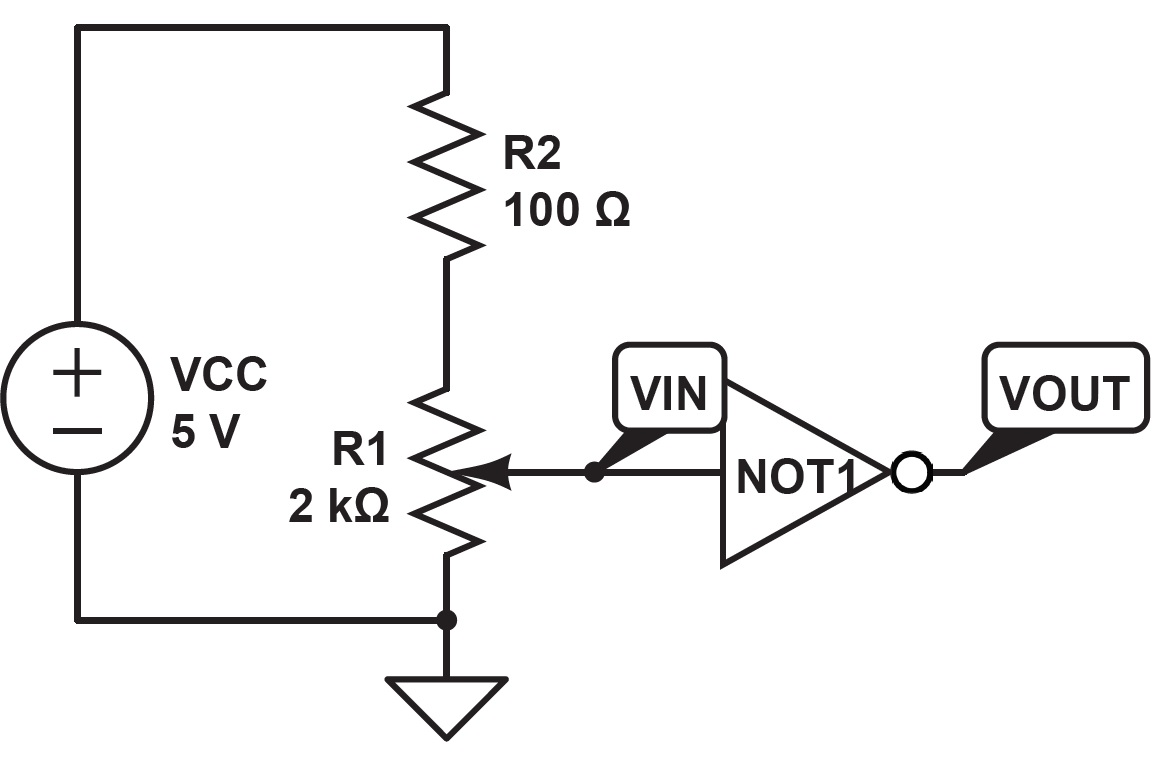
\includegraphics[scale=1.0]{../Figs-Tabs/immagine1.png}
			\caption{Rappresentazione del primo circuito impiegato.}
			\label{f:c1}
		\end{figure} ,
	dopodiché si è andati a  campionare la tensione in uscita, $V_{out}$, in funzione della tensione di ingresso , $V_{in}$.
	
	Il circuito in  \figurename{ \ref{f:c1}} permette la variazione di  $V_{in}$ variando la resistenza del trimmer $R_{1}$;infatti esso  rappresenta un partitore di tensione.
	
		Per la costruzione circuitale sono state impiegate: un trimmer $R_{1}$ di valore massimale $R_{1}^{max}=$\SI{94.0 \pm 0.8 }{\kilo \ohm} ed na resistenza $R_{2}=$\SI{100.8 \pm 0.9 }{ \ohm}.
		
	Si riportano i dati campionati in \tablename{ \ref{t:1}}
		\begin{table}[hb]
		\centering
		\begin{tabular}{|s|s|}
			\toprule
			V_{in} [\si{\volt}] & 	V_{out} [\si{\volt}]\\
			\midrule
		 0	\pm 1e-3 & 4.38 \pm 0.02\\
			0.265 \pm 0.002 & 4.23 \pm 0.02\\
			0.584 \pm 0.003 & 4.02 \pm 0.02\\
			0.780 \pm 0.004 & 3.87 \pm 0.02\\
			0.881 \pm 0.005 & 3.78 \pm 0.02\\
			0.945 \pm 0.005 & 3.44 \pm 0.02\\
			1.003 \pm 0.005 & 2.95 \pm 0.02\\
			1.065 \pm 0.006 & 2.01 \pm 0.01\\
			1.103 \pm 0.008 & 0.1773 \pm 0.009\\
			1.238 \pm 0.009 & 0.1728 \pm 0.009\\
			1.56 \pm 0.01 & 0.1728 \pm 0.009\\
			1.775 \pm 0.02 & 0.1728 \pm 0.009\\
			1.991 \pm 0.02 & 0.1727 \pm 0.009\\
			2.52 \pm 0.02 & 0.1727 \pm 0.009\\
			3.02 \pm 0.02 & 0.1726 \pm 0.009\\
			3.48 \pm 0.02 & 0.1726 \pm 0.009\\
			3.93 \pm 0.02 & 0.1726 \pm 0.009\\
			5.00 \pm 0.03 & 0.1726 \pm 0.009\\
			\bottomrule
		\end{tabular}
		\caption{Si riportano i valori corrispondenti alle nostre acquisizioni.I dati campionati sono stati ottenti col multimetro digitale.
		Si è associato alle misure l'incertezza di un  digit sulla prima cifra che risultasse instabile sommata in quadratra con eventali errori di calibrazione del mltimetro.}
		\label{t:1}
	\end{table}
	.
	Effettando un grafico  ( \figurename{ \ref{f:i1}} )
	 dei dati in  \tablename{ \ref{t:1}}, ( a cui sono stati scorporati gli errori di calibrazione del multimetro essendo uniformi per le scale impiegate) si osservano i valori di :\\
	 $V_{I,H}$, tensione in ingresso associata all'uscita HIGH;\\
	 $V_{I,L}$, tensione in ingresso associata all'uscita LOW;\\
	 $V_{O,H}$, tensione in uscita  associata all'uscita HIGH;\\
	 $V_{O,L}$, tensione in uscita associata all'uscita LOW.\\
	 
	 Essendo tali valori da intendersi come intervalli di tensione si sono osservati i loro valori superiori ed inferiori ottenendo :
	 \begin{center}
	 $V_{I,H}^{max}\sim$\SI{0}{\volt} \\
	 $V_{I,H}^{min}=$\SI{1.003 \pm 0.005}{\volt}\\
	 $V_{I,L}^{max}=$\SI{5.00 \pm 0.03}{\volt}\\
	 $V_{I,L}^{min}=$\SI{1.108 \pm 0.008}{\volt}\\
	 
	 $V_{O,H}^{min}=$\SI{2.95 \pm 0.02}{\volt}\\
	 $V_{O,H}^{max}=$\SI{4.38 \pm 0.02}{\volt}\\
	 $V_{O,L}^{min}=$\SI{0.1726 \pm 0.0009}{\volt}\\
	 $V_{O,L}^{max}=$\SI{0.1773 \pm 0.0009}{\volt}	\\
	 \end{center}
	 
	 Tali stime risultano essere meno restrittive dei  valori
	  forniti dal costruttore nel datasheet:
	   \begin{center}
	  	
	  	$V_{O,H}^{min,atteso}=$\SI{2.4}{\volt}\\
	  	$V_{O,L}^{max,atteso}=$\SI{0.4}{\volt}\\
	  	$V_{I,H}^{min,atteso}=$\SI{2}{\volt}\\
	  	$V_{I,L}^{max,atteso}=$\SI{0.8}{\volt}.\\
	  \end{center}
	  Si imputa che questa lieve discrepanza 
	 con i valori attesi, sia dovuta al fatto che essi siano misurati nelle peggiori condizioni di operatività possibili della porta NOT.
	
	 Durante la fase di presa dati è stato osservato inoltre che nella regine di tensione compresa tra 	$V_{I,L}^{max}$ ed $V_{I,H}^{min}$ il segnale in uscita, risultasse variare tra lo stato HIGH e LOW,senza un apparente continuita.
	 Questo effetto risulta compatibile col fatto che il NOT non sia forzato ne nella regione $V_{O,H}$ ne in $V_{O,L}$; pertanto  l'uscita risulta indeterminata tra il regime di uscita high e low.
	\begin{center}
		\begin{figure}[h]
			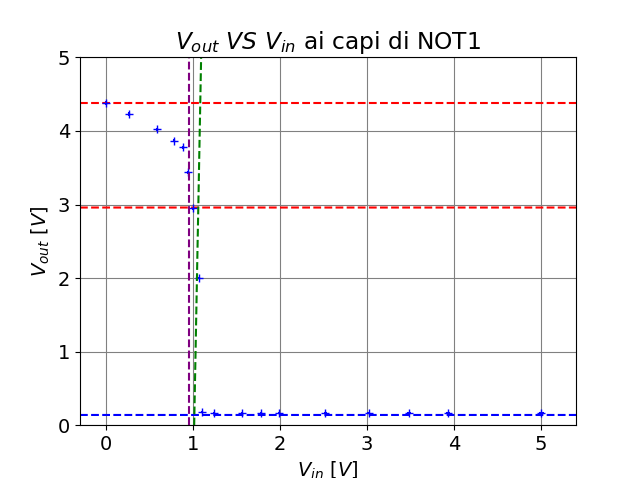
\includegraphics[scale=0.50]{../Figs-Tabs/in-ot2.png}
			\caption{Rappresentazione dei dati in \tablename{ \ref{t:1}}.}
			\label{f:i1}
		\end{figure}
	\end{center}

	
\section{Montaggio arduino}
	Per la verifica delle caratteristiche dinamiche dell'IC SN74LS244 si è montato un circito impulsatore, basato su di un microcontrollore arduino; successivamente impiegato come generatore di onde. 
	
	Si riporta lo schema circitale in \figurename{ \ref{f:impulsatore}}. 
	
		\begin{figure}[htb]
			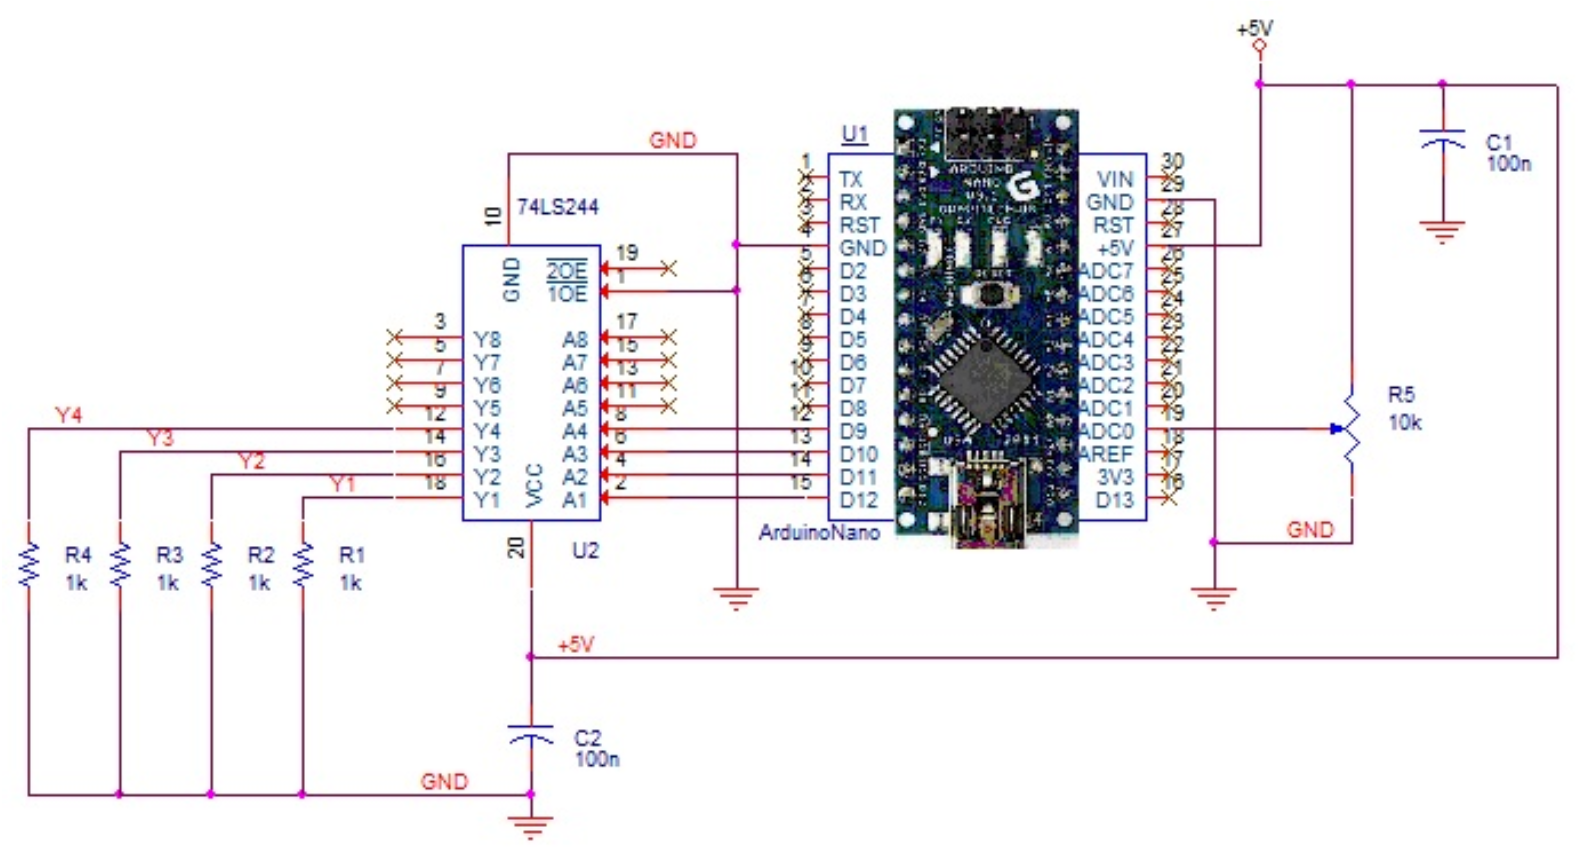
\includegraphics[scale=0.50]{../Figs-Tabs/imp.png}
			\caption{Rappresentazione del circuito impulsatore montato.}
			\label{f:impulsatore}
		\end{figure}
	Per il montaggio sono state impiegate le  segenti componenti circitali:
	\begin{center}
	\bigskip
		$R_{1}=$\SI{984 \pm 8}{\ohm} $R_{2}=$\SI{984 \pm 8}{\ohm} $R_{3}=$\SI{982 \pm 8}{\ohm} \\
		$R_{4}=$\SI{983 \pm 8}{\ohm} n trimmer di $R_{5}^{max}=$\SI{10.2 \pm 0.8}{\kilo \ohm} \\
 		dei condensatori	$C_{1}=$\SI{114 \pm 6 e-9}{\farad} $C_{2}=$\SI{114  \pm 6 e-9}{\farad}
	
	\end{center}
	Si segnala inoltre 
	che da questa sezione si è impiegata una tensione di alimentazione $V_{cc}=$\SI{4.87 \pm 0.03}{\volt}; tale accorgimento è stato impiegato per evitare di danneggiare il microcontrollore arduino, sensibile per tensioni superiori a \SI{5}{\volt}.

	Il circuito montato tra i terminali Y1 e Y2 dovrebbe generare delle onde quadre sfasate di $\pi/2$ , di frequenza regolabile attraverso il valore di $R_{5}$, e  compresa tra 50 Hz e 50KHz.
	
	Si è andati pertanto a verificarne il corretto montaggio attraverso la verifica di queste proprietà.
	Attraverso l'oscilloscopio si sono visalizzati su ch1 la tensione rilevata su Y1 e su  ch2 la tensione letta su Y2. Si riporta una tipica acquisizione in 
	\figurename{ \ref{f:oscil} }.
	\begin{figure}[htb]
		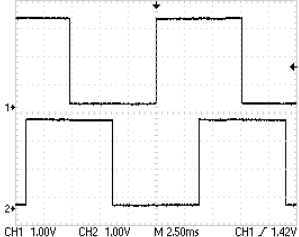
\includegraphics[scale=0.50]{../Figs-Tabs/ondaquadra_esempio.png}
		\caption{Tipica acqisizione delle tensioni lette si terminali Y1 (ch1) e Y2 (ch2) del circuito impulsatore.}
		\label{f:oscil}
	\end{figure}

	Come è possibile osservare dall'acquisizione la forma d'onda presentata dalle due tracce può essere trattata quale un onda quadra; si osserva inoltre che al variare del valore della resistenza $R_{5}$ la frequenza delle tracce assume valori compresi nell'intervallo $f\in [\sim 10 \text{Hz;} \sim 50 \text{KHz}]$.
	
	Come ultima verifica dell'operatività del circuito montato si e proceduto a misurare lo sfasamento tra le due tracce.
	Per fare ciò si è andati a misurare il $\Delta t$ tra i fronti di salita delle dei due canali, ottenendo $\Delta t=$\SI{248 \pm 2}{\mu \sec}\footnote{misura effettuata con i cursori dell'oscilloscopio in dotazione.} a fronte di una frequenza
	  $f=$\SI{1.007 \pm 0.001}{\kilo \hertz}\footnote{la misura di frequenza è stata effettuata con la funzione di lettura automatica dell'oscilloscopio; a cui abbiamo abbiamo associato l'incertezza di un digit sulla cifra precedente alla prima che risultasse instabile. } .
	Essendo valida la relazione \begin{equation}
	\Delta \phi = 2 \pi \cdot f \cdot \Delta t
	\end{equation}\label{eq:sfas}
	si ottiene $\Delta \phi=$\SI{1.57 \pm 0.01 }{\radian} ,compatibile con $\phi/2$.
	
	Visto l'accordo tra le richieste operative ed il funzionamento del circuito impulsatore montato 
	si è assunto  come  corretta la realizzazione dello stesso.
	

	\end{document}
	
	